%!TEX root = ../../../main.tex

\subsection{Multi-view Analysis Algorithms}

    The goal of multi-view analysis algorithms is to construct a common low-dimensional embedding that should preserve sufficient information or even be more informative than each individual view.

    Let's define $X = \{x_{ijk}|i=(1,..,c);j = (1,..,v);k=(1,..,n_{ij})\}$ as samples from $v$ views where $x_{ijk} \in R^{d_j}$ is the $k^{th}$ sample from the $j^{th}$ view of the $i^{th}$ class, $d_j^x$ is the original dimension of data at the $j^{th}$ view and $d^y$ is the dimension of common space such that $d^y < \sum_{j=1}^{v}{d_j^x}$.
    Different methods for features extraction from single view have been presented in previous sections. 

    \subsubsection{Multi-view discriminant analysis}
        Multi-view discriminant analysis (MvDA) is an extension of LDA for multi-view scenario \cite{kan2015multi}.
        It tries to determine a set of $v$ linear transformations to project all action samples from each view $j = (1,..,v)$ to a common space.
        The projection results of $X$ on the common space is denoted by $Y = \{y_{ijk} = w_j^T x_{ijk}|i=(1,..,c); j=(1,..,v); k=(1,...,n_{ij})\}$.
        The common space is built by maximizing the between-class variation $\boldsymbol{S}_B^y$ while minimizing the within-class variation $\boldsymbol{S}_W^y$ from all views. $\boldsymbol{S}_B^y$ and $\boldsymbol{S}_W^y$ are computed as follows: 

        \begin{align}
            \boldsymbol{S}_W^y &= \sum_{i=1}^{c}\sum_{j=1}^{v}\sum_{k=1}^{n_{ij}}(y_{ijk}-\mu_i)(y_{ijk}-\mu_i)^T \label{eq:MvDA_Sw}\\
            \boldsymbol{S}_B^y &= \sum_{i=1}^{c}n_i(\mu_i - \mu)(\mu_i - \mu)^T \label{eq:MvDA_Sb}
        \end{align}

        where $\mu_i=\frac{1}{n_i}\sum_{j=1}^{v}{\sum_{k=1}^{n_{ij}}}{y_{ijk}}$ is the mean of all samples of the $i^{th}$ class from all views in the common space; $\mu=\frac{1}{n}\sum_{i=1}^{c}\sum_{j=1}^{v}{\sum_{k=1}^{n_{ij}}{y_{ijk}}}$ is the mean of all samples of all classes from all views in the common space; $n=\sum_{i=1}^{c}n_i$ is the total data samples from all views.

        In order to separate the unknown transformation vectors, the between-class and within-class scatter matrices are reformulated as:

        \begin{align}
            \boldsymbol{S}_W^y &= W^T \boldsymbol{S}_W^x W = W^T\left[X\left(\boldsymbol{I} - \boldsymbol{E}\right)X^T\right]W \label{eq:mvda_Sw_vec} \\
            \boldsymbol{S}_B^y &= W^T \boldsymbol{S}_B^x W = W^T\left[X\left(\boldsymbol{E} - \frac{1}{n}\boldsymbol{\mathbbm{1}}\right)X^T\right]W \label{eq:mvda_Sb_vec}
        \end{align}
        where $W = \{\omega_1,\omega_2,...,\omega_v\}$ is concatenation of transformation vectors of all views; $\boldsymbol{I} \in \mathbb{R}^{n\times n}$ is identity matrix; $\boldsymbol{\mathbbm{1}} \in \mathbb{R}^{n\times n}$ is matrix of ones; $\boldsymbol{E} \in \mathbb{R}^{n\times n}$ is a square matrix whose definition will be given in \nameref{chap:appendix}.

        Then the objective function is formulated by a Rayleigh quotient:

        \begin{align}
            (\boldsymbol{\omega}_1^*,\boldsymbol{\omega}_2^*, ..., \boldsymbol{\omega}_v^*) &= \operatorname*{argmax}_{\boldsymbol{\omega}_1, \boldsymbol{\omega}_2,..., \boldsymbol{\omega}_v}\frac{trace({S}_B^y)}{trace({S}_W^y)}\\
            \boldsymbol{W}^* &= \operatorname*{argmax}_{\boldsymbol{W}}\frac{trace(W^{T}[X\left(\boldsymbol{E} - \frac{1}{n}\boldsymbol{\mathbbm{1}}\right)X^{T}]W)}{trace(W^{T}[X\left(\boldsymbol{I} - \boldsymbol{E}\right)X^{T}]W)}
            \label{eq:MvDA}
        \end{align}

        According to \cite{kan2016multi}, the problem satisfies the optimization form of generalized eigenvalue problem and could be analytically solved through eigenvalue decomposition.
        The concatenated $\boldsymbol{W}^* = \{\boldsymbol{\omega}_1^*,\boldsymbol{\omega}_2^*, ..., \boldsymbol{\omega}_v^*\}$ could be computed using the same procedure as $\boldsymbol{\omega}^*$ in LDA by computing the eigenvalues and eigenvectors of $\boldsymbol{S} = {\boldsymbol{S}_W^x}^{-1}\boldsymbol{S}_B^x$.
        Then, the output matrix $\boldsymbol{W}^*$ of shape $(\sum_{j=1}^{v}{d_j^x} \times d^y)$ is splitted vertically by the original dimension $d_j^x$ to get the final transformation vector $\boldsymbol{\omega}_j^*$ of shape $(d_j^x \times d^y)$ for each $j^{th}$ view (Figure \ref{fig:mvda_solution}).
        Similarly, MvDA can be used as a dimensionality reduction algorithm by choosing $d^y$ eigenvectors corresponding to $d^y$ leading eigenvalues if $d^y < d_j^x \forall j \in (1, ..., v)$.

        \begin{figure}[htbp]
            \centering
            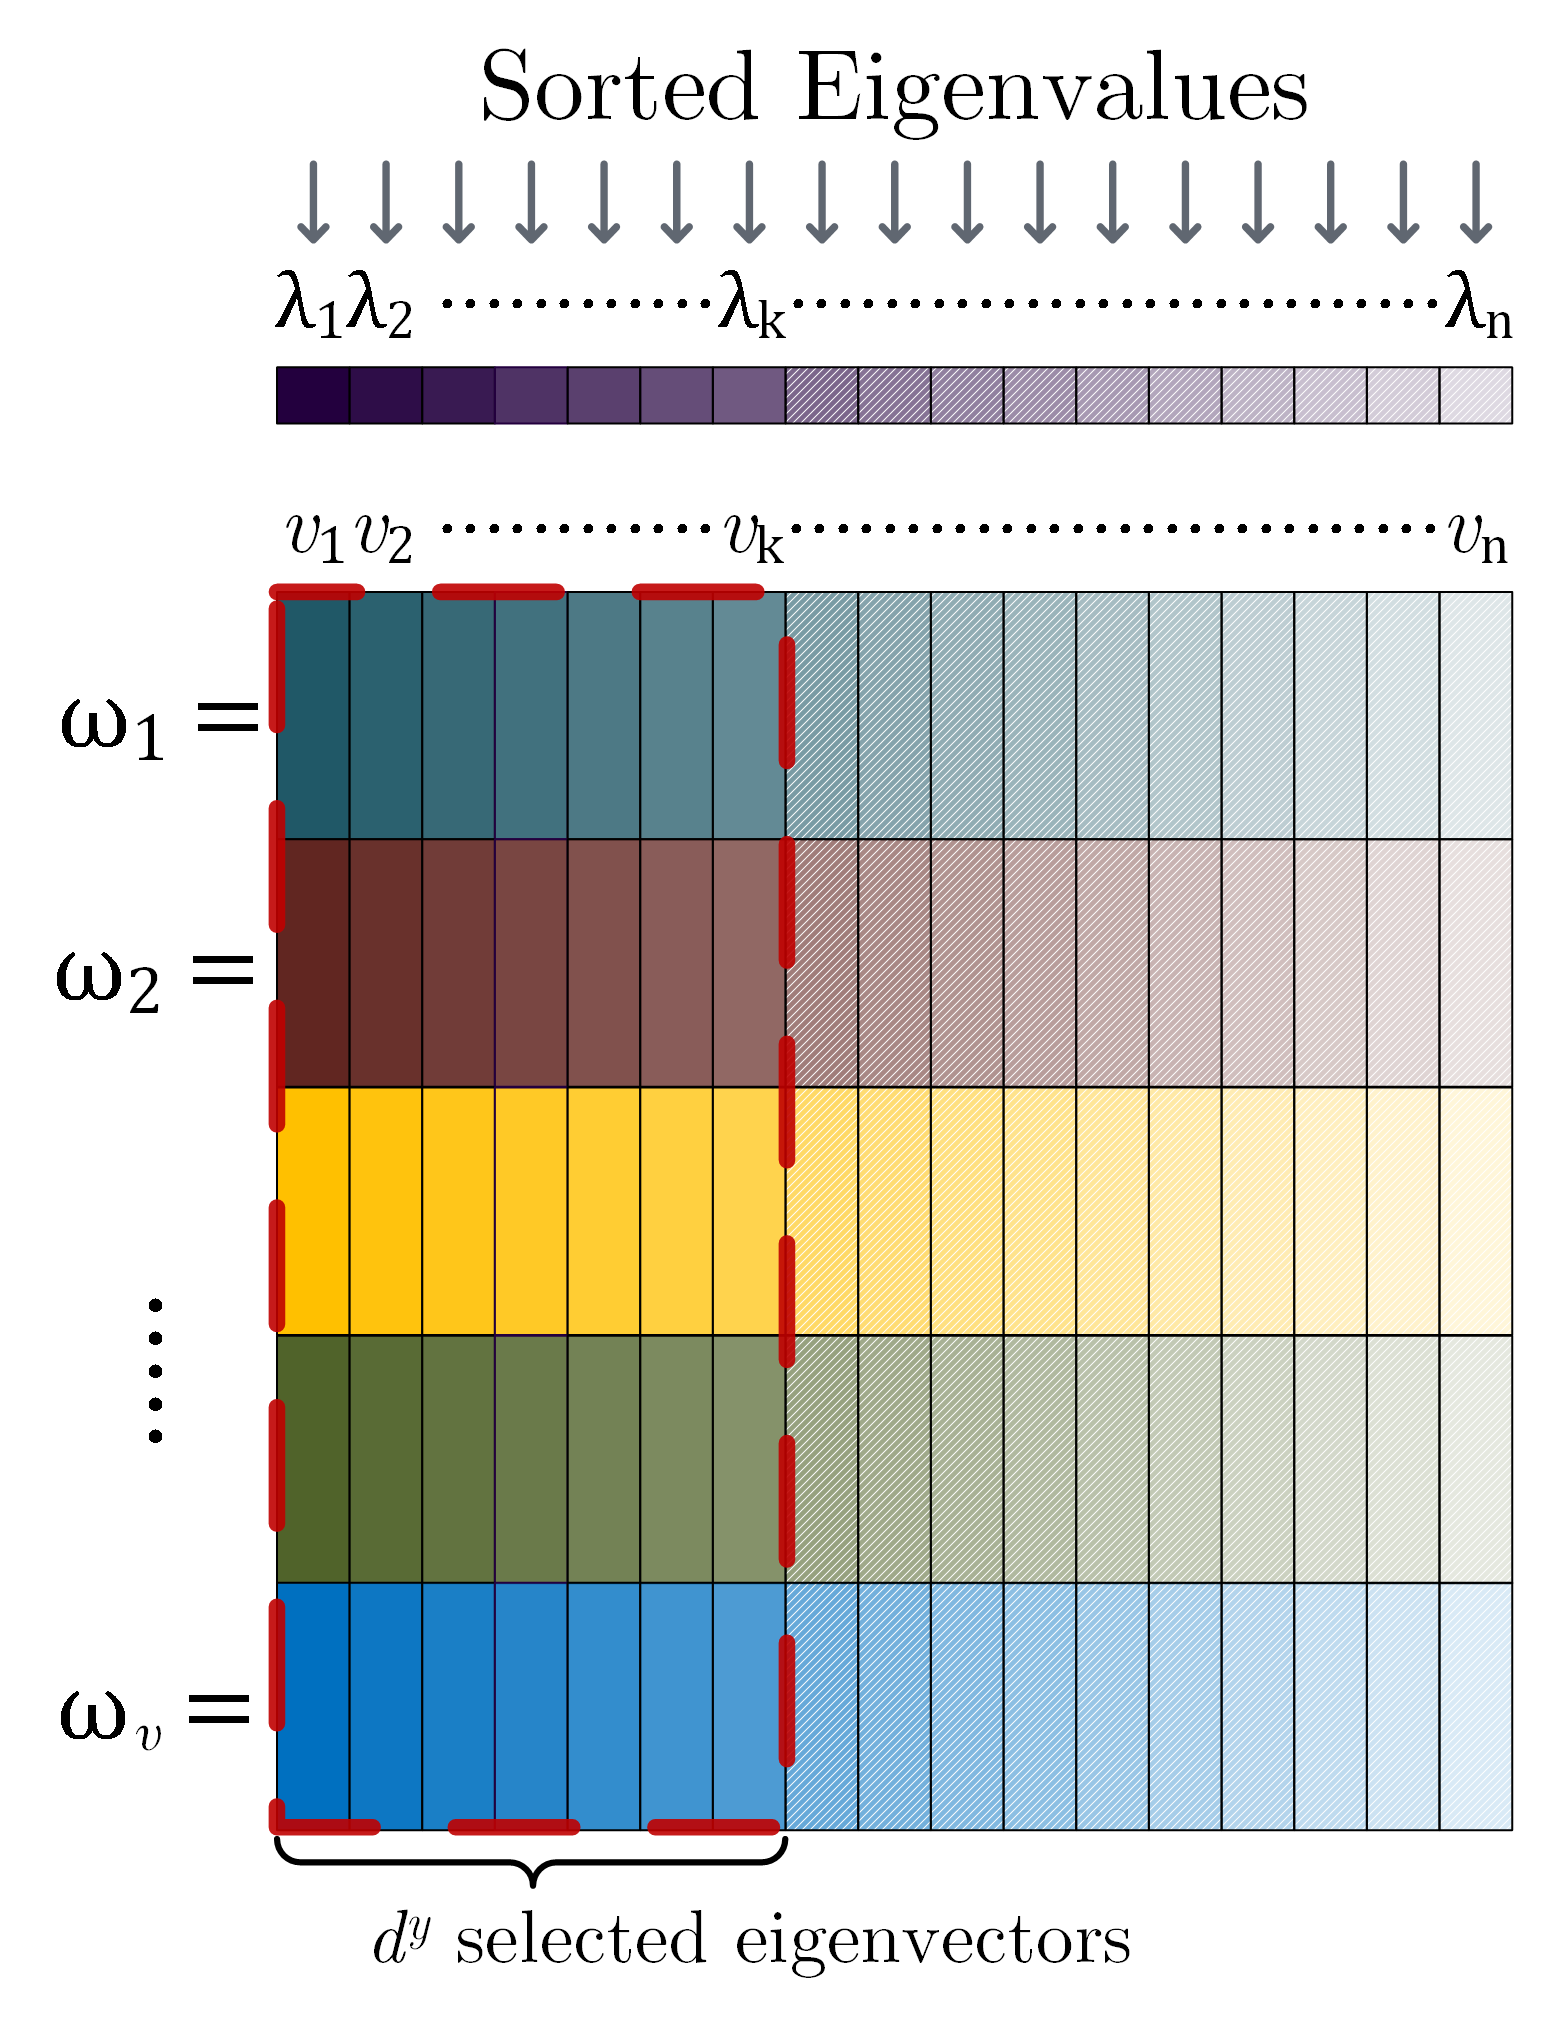
\includegraphics[width=0.4\linewidth]{figs/mvda_solution.png}
            \caption{Analytical solution of MvDA.}
            %\vspace{-0.3cm}
            \label{fig:mvda_solution}
        \end{figure}

    \subsubsection{Multi-view discriminant analysis with view-consistency} \label{subsubsec:mvdavc}

        In \cite{kan2016multi}, the authors observed that as multiple views correspond to the same objects, there should be some correspondence between multiple views.
        They then introduce a view consistency constraint into the objective function, that means if $X_j, X_r$ are observed at $j^{th}$ and $r^{th}$ views, there exists a certain transformation $\boldsymbol{R}$ such that $X_j = \boldsymbol{R}X_r$.
        As a result, the transformations obtained from two views (i.e. the projection of features extracted from singe view to common view) should have similar relationship: ${\omega}_j = \boldsymbol{R}{\omega}_r$.
        Let's define $\boldsymbol{\beta}_j$ that captures the structure of the transformation ${\omega}_j$.

        \begin{equation}
            \omega_j = X_j\boldsymbol{\beta}_j
            \label{eq:MvDA-vc_beta}
        \end{equation}

        Then the $\boldsymbol{\beta}_j$ and $\boldsymbol{\beta}_r$ capturing the structures of two transformations of two views $j$ and $r$ should be identical ${\boldsymbol{\beta}}_j = {\boldsymbol{\beta}}_r$.

        Generalizing to $v$ views, suppose that ${\boldsymbol{\beta}}_j, j=(1,..,v)$ captures the structures of $v$ transformations ${w}_j$.
        Following the above observation, the $\boldsymbol{\beta}_r, r=(1,..,v)$ should resemble mutually.
        That means the similarity between the pair of $\boldsymbol{\beta}_j$ and $\boldsymbol{\beta}_r$ should be minimized.
        The objective of view-consistency is defined as:

        \begin{equation}
            \boldsymbol{O}_{view-consistency} = \sum_{j=1}^{v}\sum_{r=1}^{v}\left|\left|\boldsymbol{\beta}_j - \boldsymbol{\beta}_r\right|\right|_2^2
            \label{eq:MvDA-vc_vc}
        \end{equation}

        From Equation \eqref{eq:MvDA-vc_beta}, we have:

        \begin{equation}
            \boldsymbol{\beta}_j = {\left(X_j^T X_j\right)}^{-1}X_j^T\omega_j \triangleq \boldsymbol{P}_j w_j
        \end{equation}

        Replacing in Equation \eqref{eq:MvDA-vc_vc} we can reformulate it as:

        \begin{equation}
            \sum_{j,r=1}^{v}||\boldsymbol{\beta}_j - \boldsymbol{\beta}_r||_2^2 = trace\left(W^{T}\boldsymbol{P}^{T}\left(2v\boldsymbol{I} - 2\boldsymbol{\widehat{I}}\right)\boldsymbol{P}W\right)
        \end{equation}
        where $\boldsymbol{P} = \{\boldsymbol{P}_1,\boldsymbol{P}_2,...,\boldsymbol{P}_v\}$; $\boldsymbol{I} \in \mathbb{R}^{n\times n}$ is identity matrix; $\boldsymbol{\widehat{I}} \in \mathbb{R}^{n\times n}$ is grid stack of identity matrices $I \in \mathbb{R}^{\frac{n}{v}\times\frac{n}{v}}$.
        This term is called in \cite{kan2016multi} {\itshape view consistency} and will be added to the denominator of Equation \eqref{eq:MvDA} for minimization.

        \begin{align}
            (\boldsymbol{\omega}_1^*,\boldsymbol{\omega}_2^*, ..., \boldsymbol{\omega}_v^*) &= \operatorname*{argmax}_{\boldsymbol{\omega}_1, \boldsymbol{\omega}_2,..., \boldsymbol{\omega}_v}\frac{trace({S}_B^y)}{trace({S}_W^y) + \alpha\sum_{j,r=1}^{v}||\boldsymbol{\beta}_j - \boldsymbol{\beta}_r||_2^2}\\
            \boldsymbol{W}^* &= \operatorname*{argmax}_{\boldsymbol{W}}\frac{trace\left(W^{T}\left[X\left(\boldsymbol{E} - \frac{1}{n}\boldsymbol{\mathbbm{1}}\right)X^{T}\right]W\right)}{trace\left(W^{T}\left[X\left(\boldsymbol{I} - \boldsymbol{E}\right)X^{T} + 2\alpha\boldsymbol{P}^T\left(v\boldsymbol{I} - \boldsymbol{\widehat{I}}\right)\boldsymbol{P}\right]W\right)}
            \label{eq:MvDA-vc}
        \end{align}

        This optimization problem could also be analytically solved by relaxing to the trace ratio optimization problem as Equation \eqref{eq:MvDA}.
        In Equation \eqref{eq:MvDA-vc}, $\alpha$ is an empirically chosen parameter that puts a weight on the view-consistency assumption.
        When $\alpha = 0$, MvDA-vc becomes the original MvDA. 
